\documentclass[11pt,journal]{article}
%\usepackage{hyperref}
%\usepackage[breaklinks]{hyperref}
\usepackage{breakurl}
\usepackage{url}
\usepackage{listings}
\usepackage{courier}
\usepackage{amsmath}
\usepackage{graphicx}
\graphicspath{ {/home/agata/Documents/coursework/SensorNetworks/Lab4/} }
%\ifCLASSOPTIONcompsoc
% IEEE Computer Society needs nocompress option
% requires cite.sty v4.0 or later (November 2003)
\usepackage[nocompress]{cite}

%\else
% normal IEEE
\usepackage{cite}
%\fi

\hyphenation{op-tical net-works semi-conduc-tor}
\addtolength{\oddsidemargin}{-.875in}
\addtolength{\evensidemargin}{-.875in} 
\addtolength{\textwidth}{1.75in}

\addtolength{\topmargin}{-.875in}
\addtolength{\textheight}{1.75in}

\begin{document}
	\title{Sensor Networks and Mobile Data Communication, Assignment 4}
	
	\author{UID: 1690550}% <-this % stops a space
		%\protect\\
		%\thanks{}}
	
	% The paper headers



	% IEEEtran.cls defaults to using nonbold math in the Abstract.
	% This preserves the distinction between vectors and scalars. However,
	% if the journal you are submitting to favors bold math in the abstract,
	% then you can use LaTeX's standard command \boldmath at the very start
	% of the abstract to achieve this. Many IEEE journals frown on math
	% in the abstract anyway. In particular, the Computer Society does
	% not want either math or citations to appear in the abstract.
	
	% Note that keywords are not normally used for peerreview papers.
	
	% make the title area
	\maketitle
	
	
	% To allow for easy dual compilation without having to reenter the
	% abstract/keywords data, the \IEEEcompsoctitleabstractindextext text will
	% not be used in maketitle, but will appear (i.e., to be "transported")
	% here as \IEEEdisplaynotcompsoctitleabstractindextext when compsoc mode
	% is not selected <OR> if conference mode is selected - because compsoc
	% conference papers position the abstract like regular (non-compsoc)
	% papers do!
	%\IEEEdisplaynotcompsoctitleabstractindextext
	% \IEEEdisplaynotcompsoctitleabstractindextext has no effect when using
	% compsoc under a non-conference mode.
	
	
	% For peer review papers, you can put extra information on the cover
	% page as needed:
	% \ifCLASSOPTIONpeerreview
	% \begin{center} \bfseries EDICS Category: 3-BBND \end{center}
	% \fi
	%
	% For peerreview papers, this IEEEtran command inserts a page break and
	% creates the second title. It will be ignored for other modes.
	%\IEEEpeerreviewmaketitle
	\section{Part 1}
	\subsection{Question 1}
	The network topology is as follows:
	
	\begin{figure}[h]
		\centering
		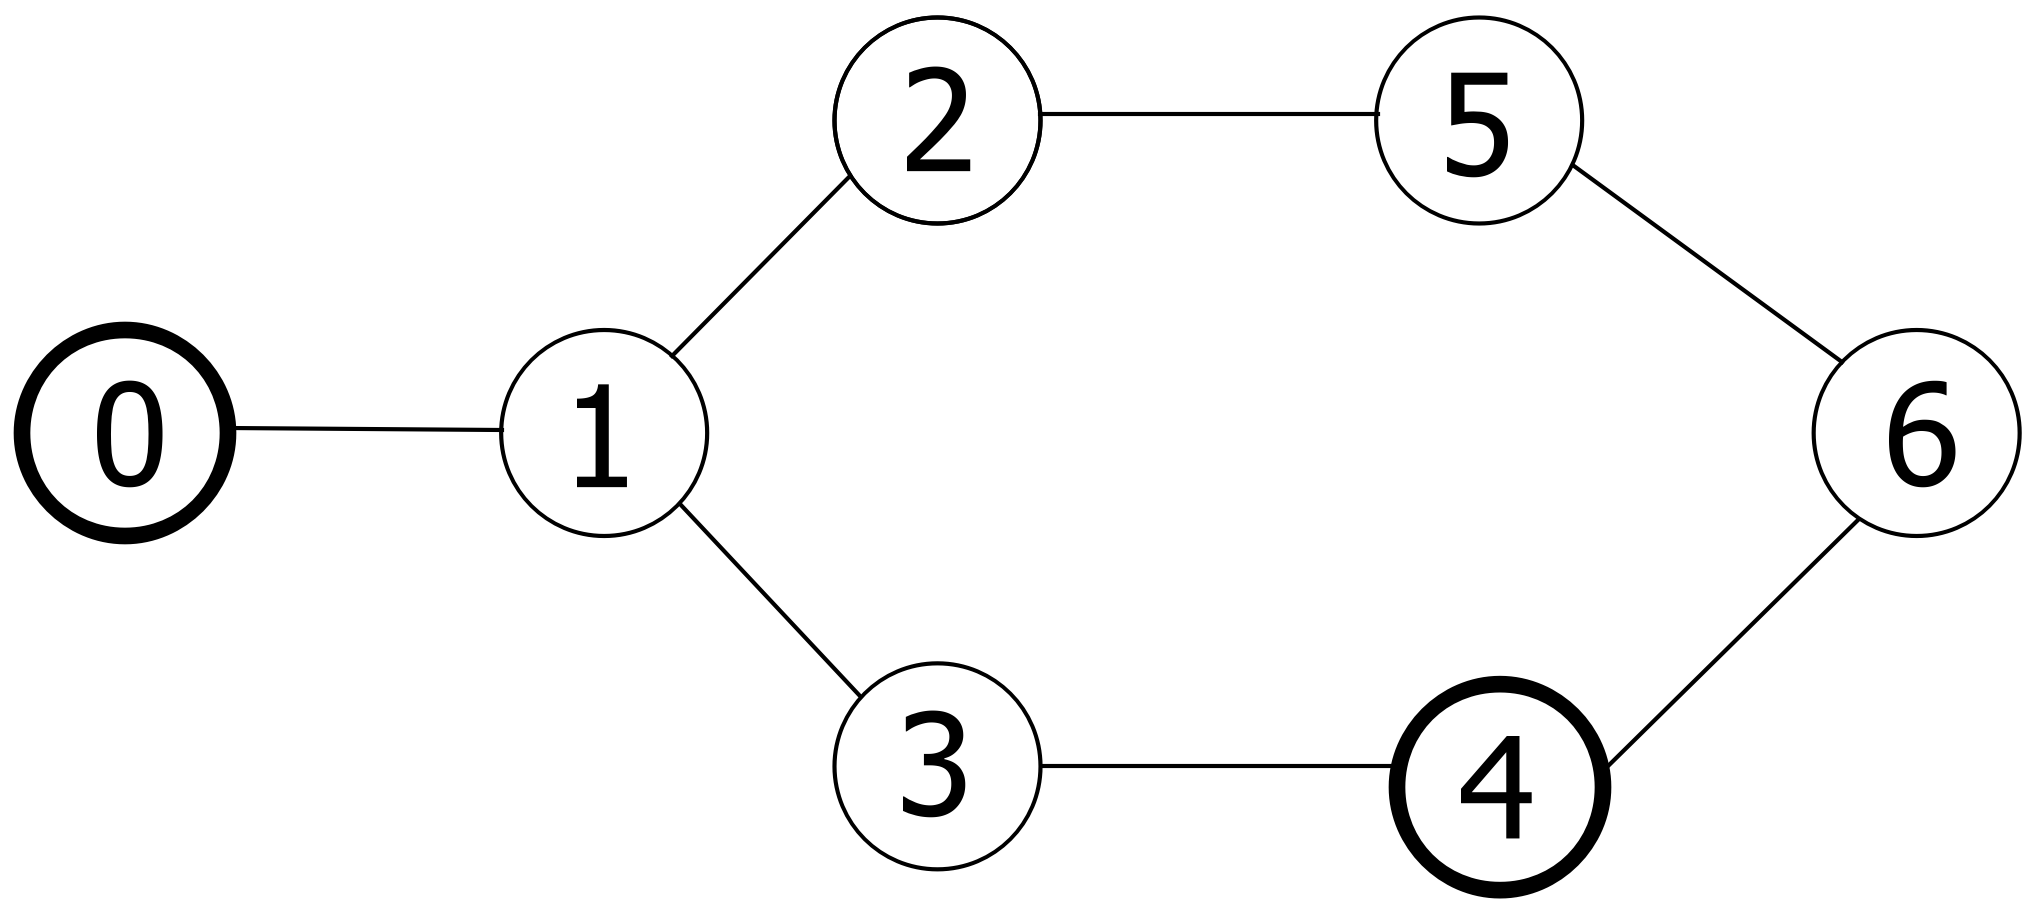
\includegraphics[scale=0.6]{lab4i_topology.png}
		\caption{Network topology, with source and destination highlighted}
	\end{figure}

	\subsection{Question 3}
	Ignoring the data link layer, the packets sent in the simulation are listed below. Bear in mind that all packets are sent in broadcast mode, and in all the route request messages, the destination node is 4.
	
	\begin{itemize}
		\item \textbf{@1.001} 0 sends out the first route request (RR) message, looking for a route to 4.
		\item \textbf{@1.00126} 1 receives that message
		\item \textbf{@1.00926} 1 sends another RR
		\item \textbf{@1.00951} this RR is received by 0, 2, and 3
		\item \textbf{@1.00956} 3 sends RR
		\item \textbf{@1.00982} this RR is received by 1 and 4 (destination node)
		\item \textbf{@1.01151} 2 sends RR (it happens to be before 4's reply, and before 2 can possibly know that the destination was discovered)
		\item \textbf{@1.01177} 1 and 5 receive 2's RR
		
		\item \textbf{@1.01273} 4 replies with route reply (RRp) that the destination was found
		\item \textbf{@1.01298} 3 and 6 receive 4's RRp
		\item \textbf{@1.01526} 3 sends RRp
		\item \textbf{@1.01551} 1 and 4 receive 3's RRp
		\item \textbf{@1.01677} 5 sends an RR
		\item \textbf{@1.01702} 2 and 6 receive 5's RR
		\item \textbf{@1.01986} 1 sends RRp, having received it from 3
		\item \textbf{@1.02012} 0, 2, and 3 get 1's RRp
		\item \textbf{@1.02502} 6 sends out an RR
		\item \textbf{@1.02528} 4 and 5 receive 6's RR
		\item 4 does not reply to 6's RR, because it is older than it's current sequence
		\item 6's message times out
		\item \textbf{@1.03025} 0 sends out the Payload, having received RRp
		\item \textbf{@1.03056} 1 receives the Payload
		\item \textbf{@1.03361} 1 sends out the Payload
		\item \textbf{@1.03392} the Payload is received by 0, 2, and 3
		\item \textbf{@1.04444} 3 sends out the Payload
		\item no other node forwards the Payload, because they are not on the route
		\item \textbf{@1.04475} 1 and 4 receive the Payload from 4. The message has reached the destination.
		
	\end{itemize}

	The simulation ends at 1.04506 s.

	\subsection{Question 4}
	Now that we want to send 2 packets, instead of 1, we observe the same process as before for the first packet. The second packet is scheduled to be send 20 s after the first one. The route timeout is set to 15 s, so we need to rediscover the route. Starting at 21.007, 0 sends another RR.
	
	This time it just so happens that 2 manages to send on the RR before 3, at 21.0185, which is received by 1 and 5 at 21.0188. 3 sends the RR at 21.0225 and it is received by 1 and 4 at 21.0228. This is sequence number 0. 4 replies immediately (same timestamp, possibly due to rounding error) with RRp. The RRp travels across the network, to reach node 0 at 21.0248.
	
	Node 0 sends the Payload 21.0252, which travels through nodes 1 and 3, and reaches 4 at 21.0269.
	
	After that 5 sends its RR to 6 (and 2) at 21.0288. 6 receives it at 21.029 and sends its RR at 21.039, but of course at this point it's quite useless, and does not get an RRp from 4.
	
	\subsection{Question 7}
	Now we schedule the breakage for 15 s and increase the timeout. The first part is the same as before, with the first Payload being received by 4 at 1.04475.
	
	20 seconds later, at 21.007 0 sends out another RR. Note that this is after the scheduled breakage. The process now goes as follows:
	
	\begin{itemize}
		\item \textbf{@21.007} 0 sends out the route request (RR) message, looking for a route to 4.
		\item \textbf{@21.0073} 1 receives that message
		\item \textbf{@21.0073} 1 sends back an RRp, which is stored and didn't time out this time
		\item \textbf{@21.0076} this RRp is received by 0, 2, and 3
		\item \textbf{@21.0084} 0, being happy with the RRp it just got, sends the Payload
		\item \textbf{@21.0087} the Payload is received by 1
		\item \textbf{@21.0091} 1 sends the Payload
		\item \textbf{@21.0094} the Payload is received by 0, 2, and 3
		\item \textbf{@21.0098} 3 sends the Payload, still believing that it has a link to 4
		\item \textbf{@21.0101} the Payload is received only by 1
		\item 3 re-sends the Payload at 21.0115, 21.0133, 21.0184, 21.0263, 21.0353, and 21.0464
		\item these 6 attempts are received only by 1
		\item \textbf{@21.0561} 3 sends a Route Error message
		\item \textbf{@21.0563} 1 receives the error message
		\item \textbf{@21.0623} 1 broadcasts the error message
		\item \textbf{@21.0626} 0, 2, and 3 receive it
		
	\end{itemize}

	The simulation ends here, and the second message never gets to 4.
	\pagebreak
	\section{Part II}
	\subsection{Question 1}
	The network topology is as shown in the figure 2 below (please note that the plot of the ranges may not be exact, but the steps of the random walk are plotted exactly):
	
	\begin{figure}[h]
		\centering
		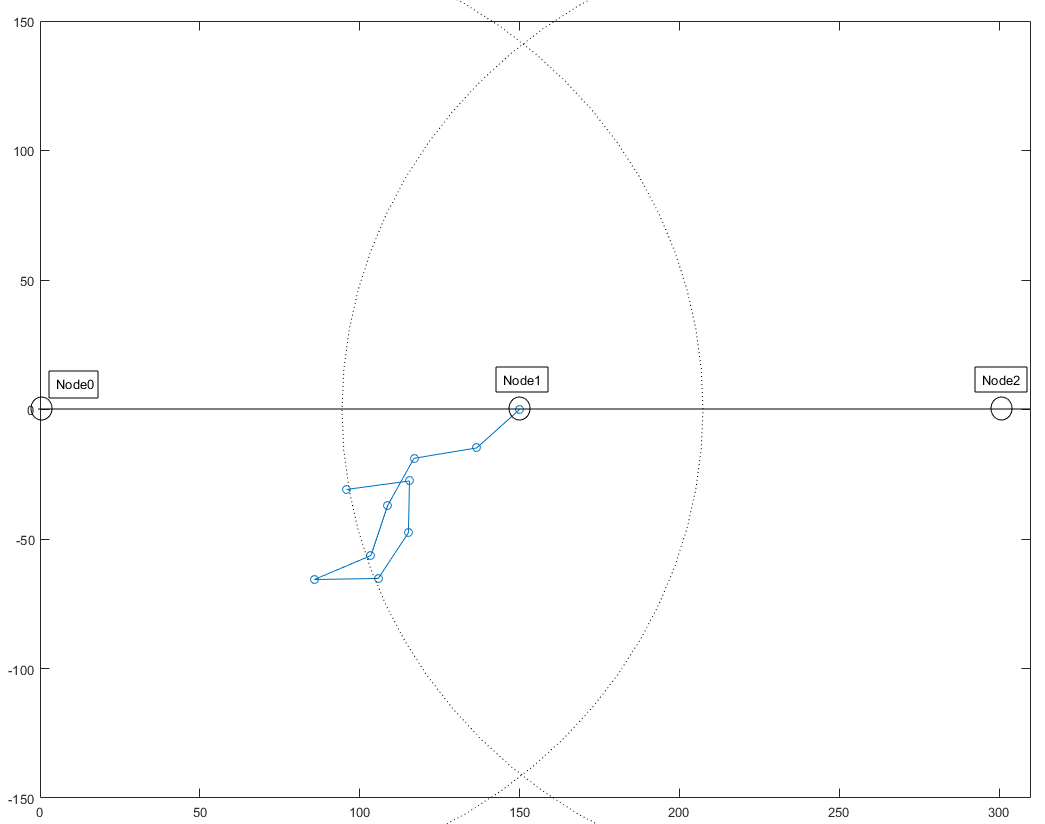
\includegraphics[scale=0.4]{lab4ii_walk_matlab.png}
		\caption{Network topology, with an example of a random walk for node 1}
	\end{figure}
	Packets are received by Node2 if and only if Node1 is in the intersection of the transmission ranges of Node0 and Node2. Node1 is neither a sink nor a source, it just acts as a relay between the two nodes.
	\subsection{Question 2}
	The values for the walk are as follows:
	\begin{table}[h]
		\centering
		\begin{tabular}{|c|c|c|c|}
			\hline
			Iteration & X & Y & Packet received by Node2\\
			\hline
			1. & 150 & 0 & Yes\\
			\hline
			2. & 136.597 & -14.8449 & Yes\\
			\hline
			3. & 117 & -18.8365 & Yes\\
			\hline
			4. & 108.762 & -37.0613 & No\\
			\hline
			5. & 103.533 & -56.3656 & No\\
			\hline
			6. & 85.8215 & -65.6554 & Yes\\
			\hline
			7. & 105.817 & -65.224 & Yes\\
			\hline
			8. & 115.241 & -47.5835 & Yes\\
			\hline
			9. & 115.583 & -27.5864 & Yes\\
			\hline
			10. & 95.8562 & -30.8748 & No\\
			\hline
		\end{tabular}
	\caption{Recorded random walk}
	
	\end{table}


	\pagebreak
	\subsection{Question 3}
	After increasing the speed of Node1 almost tenfold, the path is much more erratic. Note that the direction of Node1's movement changes every second, but now it travels much further between the changes, bouncing off the boundaries of the region.
	
	Node1 receives only 2 packages, and Node2 doesn't receive anything. This isn't surprising, as Node1 moves in and out of transmission range of either node between receiving and sending any messages.
	
	\begin{figure}[h]
		\centering
		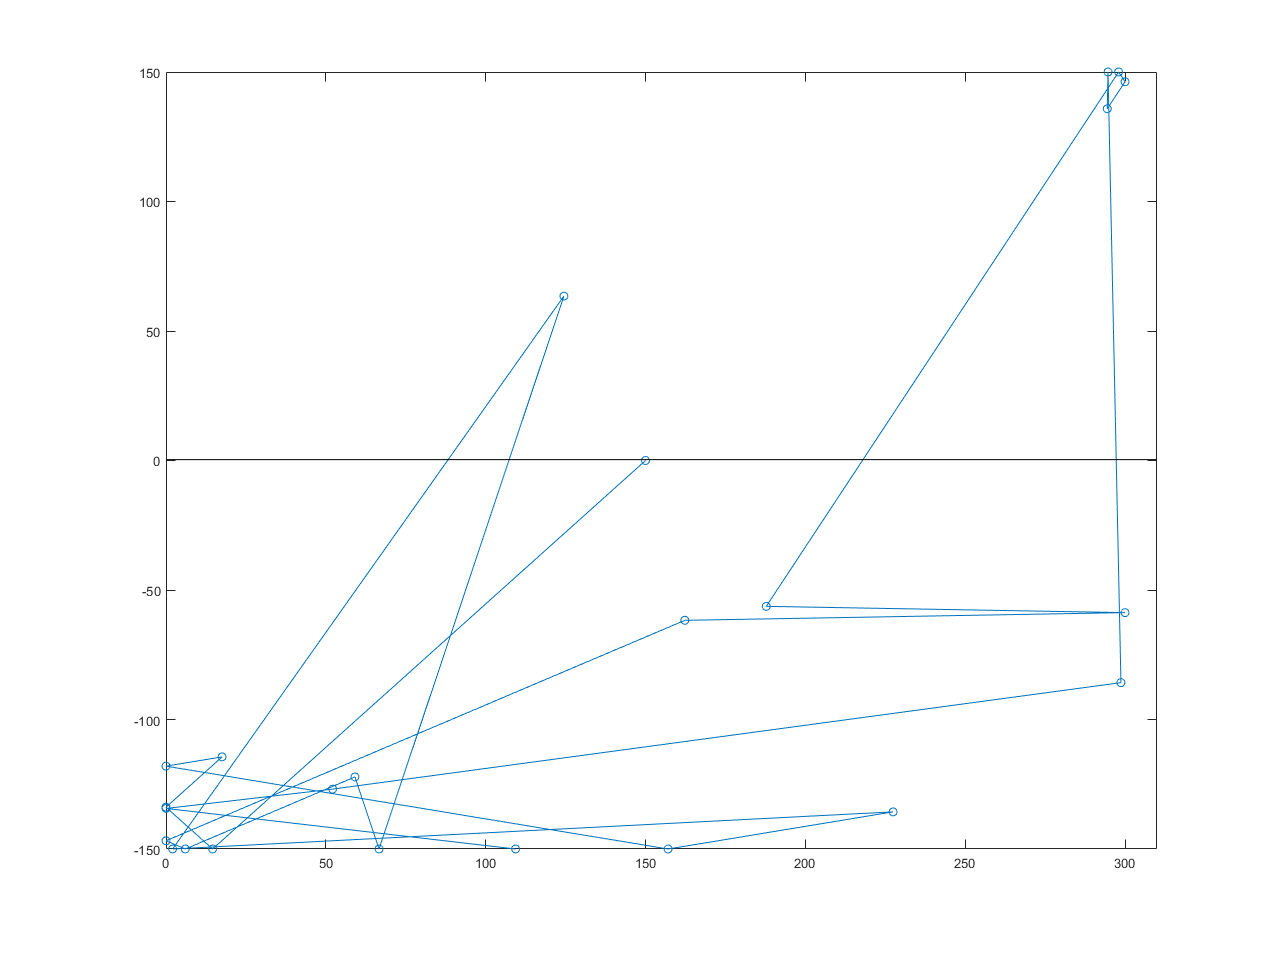
\includegraphics[scale=0.5]{lab4ii_walk_matlab2.png}
		\caption{Random walk travelled by Node1, after increasing its speed to 250 m/s}
	\end{figure}
	
	%\IEEEPARstart{}{} 
	

	
	% that's all folks
\end{document}

